This section reviews the main features of a dynamic multicore processor.
It also  briefly introduces streaming programming models and their relevance to dynamic multicore processors.

\subsection{Dynamic Multicore Processors}

% This section explains what a dynamic multicore is

Chip Multiprocessors (CMPs) have become ubiquitous due to the difficulty in scaling single core performance.
CMPs with homogeneous cores have dominated the space as they reduce the complexity of the design problem.
Yet research shows that using heterogeneous cores allows for better performance~\cite{suleman2009asymmetric}, albeit with increased design complexity. 
In both cases, once the chip is fabricated the design cannot be modified, meaning that many of the trade-offs between power, performance and area cannot be changed after production.

Dynamic Multicore Processors (DMPs) attempt to bridge the gap between the two previous designs by allowing the execution substrate to adapt dynamically at runtime.
A DMP is composed of a group of homogeneous cores (in this study) with a reconfigurable fabric.
The advantage of DMPs over the traditional CMP is the ability to reconfigure the processor to better match the tasks at hand.
For example, large sequential sections of code with high Instruction Level Parallelism (ILP) can be accelerated on a set of fused cores that mimic a wide superscalar processor.
On a parallel workload the DMP can be reconfigured by splitting the fused cores to match the Thread Level Parallelism (TLP).

\begin{figure}[t]
    \centering
    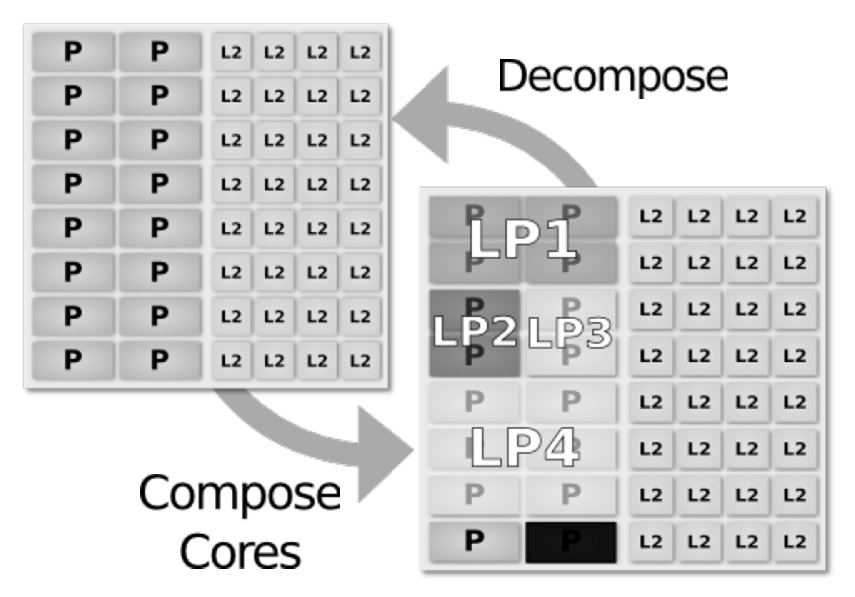
\includegraphics[width=0.3\textwidth]{streamit-paper/graphics/dmcgraph.pdf}
    \caption{High-level view of a dynamic multicore processor considered in this paper.}
    \label{fig:dynmulticore}
\end{figure}

%Explain the figure
In this paper we consider a dynamic multicore processor which allows cores to compose their execution resources, register files and private L1 caches to create logical processors to accelerate a single thread.
Figure~\ref{fig:dynmulticore} shows a high-level view of the architecture and the two possible states: composed and decomposed.
The composed state represents a set of physical cores fused to create a larger logical core.
Multiple sets of cores can be fused to create logical cores of different sizes.
In Figure~\ref{fig:dynmulticore} for example, LP1 is composed of four physical cores whereas LP2 is composed of two.
At runtime, physical cores may be decomposed from a logical processor to remove them from the core composition.

\vspace{10mm}
\subsection{Streaming Programming Languages}

% % This section should explain what steaming programming is (remove all the details about each language)
% General purpose programming languages often propose very little support for programs that handle with a continuous flow of data.
% This results in having to design a set of complicated for loops to manage the streams of data.
% Having to deal with different rates of incoming and outcoming data also increases the complexity of writing these applications using a standard language.

Streaming programming languages are a branch of dataflow programming that focus on applications that deal with a constant stream of data.
These applications, such as audio or video decoding can be commonly found in mobile devices.
Unlike conventional programming languages such as C++, these languages abstract the concept of incoming and outgoing data to permit the programmer to focus on how the data should be treated.
Programs are described as directed graphs where nodes are functions and their edges represent their input and output streams. 
These languages offer primitives to describe such a graph~\cite{theis2002streamit} which expose parallelizable and serial sections of the application directly to the compiler. 
Rates of incoming and outcoming data can also be defined to facilitate load balancing optimizations~\cite{chen2005rawstream}.

Features of streaming programming languages make them an ideal language for targeting multicore processors.
The explicit data communication between the different tasks in the program, the ability to estimate the amount of work performed in each task and information about data rates between tasks allows the compiler to easily generate a multi-threaded application that can run on a dynamic multicore processor.
However, the main challenge consists of deciding how to map the different tasks onto threads and how to allocate the right amount of resources to maximize performance.

